\section{System Architecture}

\begin{figure}[!htbp]
\begin{mdframed}
    \centering
    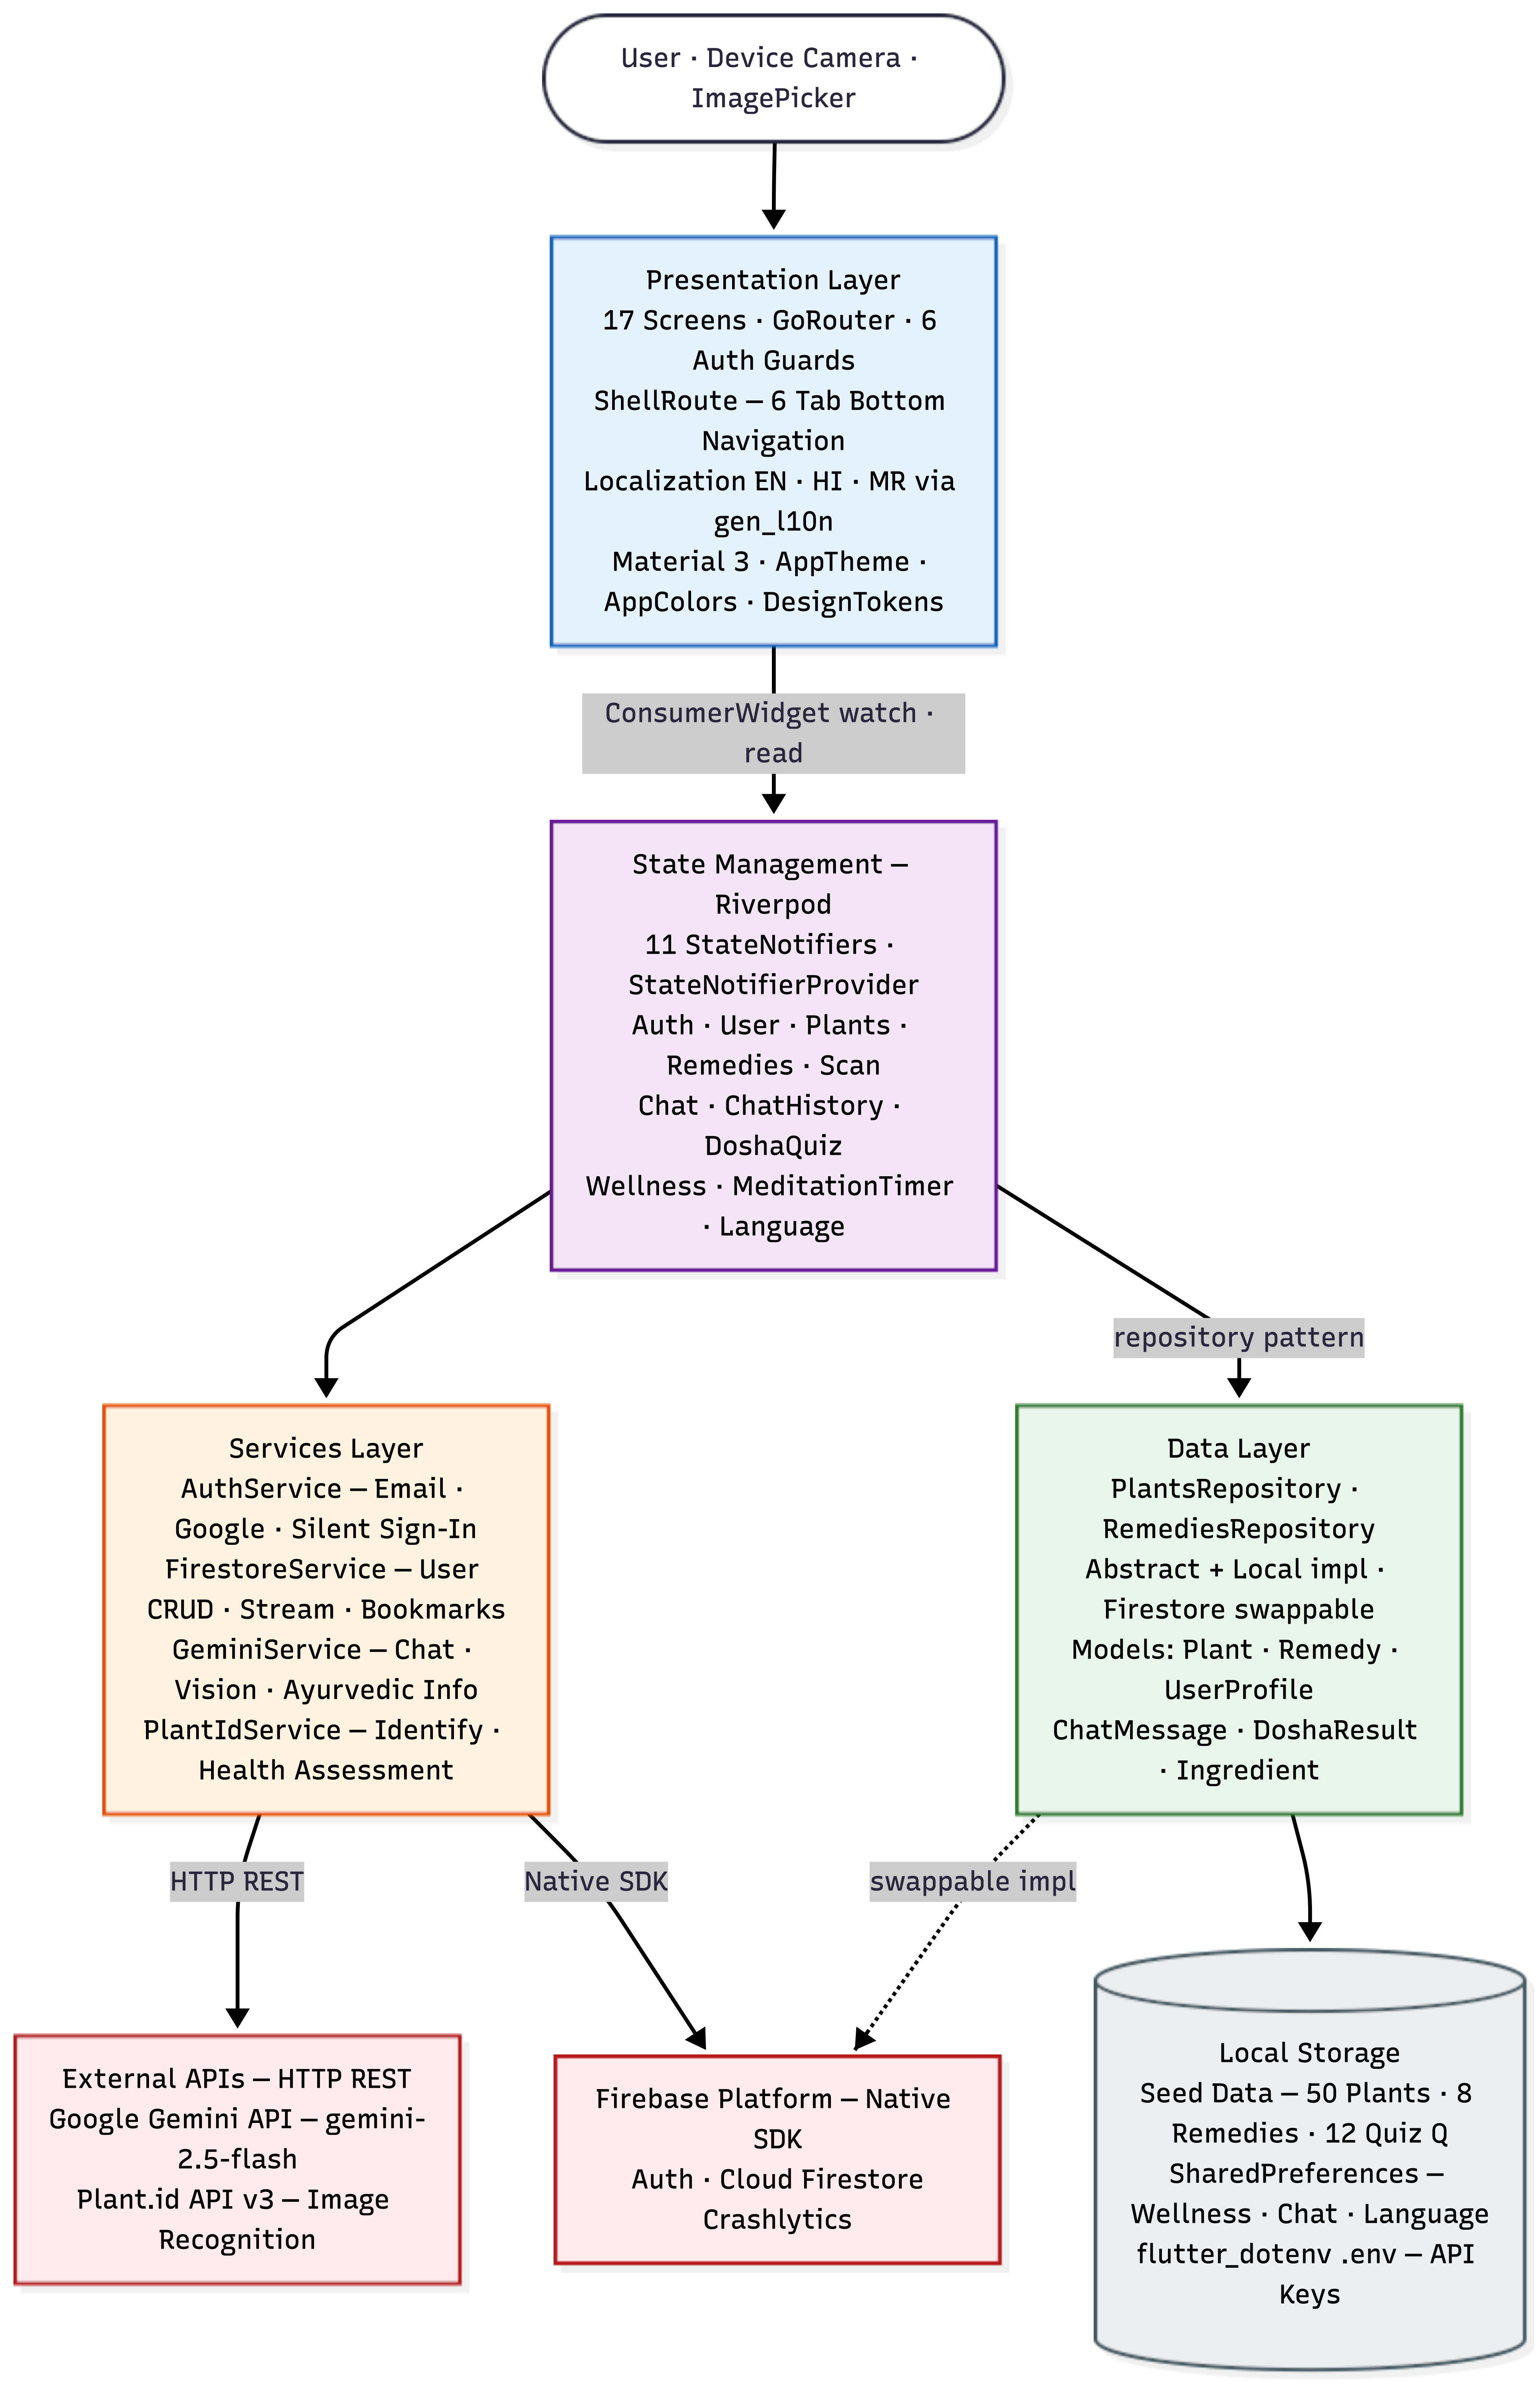
\includegraphics[width=0.7\linewidth,keepaspectratio]{assets/placeholders/placeholder_system_arch.png}
\end{mdframed}
\caption{Implemented System Architecture}
\end{figure}

\justify
High-resolution images (12MP) incur payload cost in network transmissions. A local
Pre-processing function $P(I_{raw})$ performs bicubic downsampling to JPEG Q=85,
decreasing payloads by 84\% before interfacing with REST APIs.

The dual-stage API pipeline (Hybrid Inference) uses Plant.id for discriminative visual
confidence and Gemini for generative Ayurvedic reasoning. Specific System Prompts acting
as `AyurBot' curb ``Alignment Drift.'' Riverpod manages asynchronous state updates
across independent threads, ensuring efficiency on affordable hardware.

\newpage
\section{State Management with Riverpod}
\justify
Riverpod provides compile-time safe global state management. The \texttt{ChatState}
manages message history, loading states (typing indicators), and errors:

\begin{lstlisting}[language=C++]
class ChatState {
  final List<ChatMessage> messages;
  final bool isTyping;
  final String? error;

  const ChatState({
    this.messages = const [],
    this.isTyping = false,
    this.error,
  });

  ChatState copyWith({
    List<ChatMessage>? messages,
    bool? isTyping,
    String? error,
    bool clearError = false,
  }) {
    return ChatState(
      messages: messages ?? this.messages,
      isTyping: isTyping ?? this.isTyping,
      error: clearError ? null : (error ?? this.error),
    );
  }
}
\end{lstlisting}

Providers by domain:
\begin{itemize}
    \item \textbf{AuthProvider}: Firebase Authentication state management.
    \item \textbf{ScanProvider}: Image capture and Plant.id processing pipeline.
    \item \textbf{DoshaQuizProvider}: Step-by-step \textit{Prakriti} calculation state.
    \item \textbf{UserProvider}: Firestore profile synchronization.
\end{itemize}

\section{External AI Integrations}

\subsection{API Configuration}
\begin{lstlisting}[language=C++]
import 'package:flutter_dotenv/flutter_dotenv.dart';

class ApiConfig {
  ApiConfig._();
  static String get plantIdApiKey =>
      dotenv.env['PLANT_ID_API_KEY'] ?? '';
  static const String plantIdBaseUrl =
      'https://plant.id/api/v3';
  static String get geminiApiKey =>
      dotenv.env['GEMINI_API_KEY'] ?? '';
  static const String geminiModel = 'gemini-2.5-flash';
  static bool get isPlantIdConfigured =>
      plantIdApiKey.isNotEmpty &&
      plantIdApiKey != 'YOUR_PLANT_ID_API_KEY';
  static bool get isGeminiConfigured =>
      geminiApiKey.isNotEmpty &&
      geminiApiKey != 'YOUR_GEMINI_API_KEY';
}
\end{lstlisting}

\subsection{Plant.id Integration}
The \texttt{PlantIdService} communicates with Kindwise Plant.id API via REST/HTTP. It
maps the deeply nested JSON response to the \texttt{PlantIdResult} Dart object,
abstracting JSON structure from the rest of the application.

\subsection{Google Gemini Integration}
AyurSpace uses \texttt{gemini-2.5-flash} for high inference speed and multimodal
capabilities. The \texttt{GeminiService} provides:
\begin{itemize}
    \item \texttt{getAyurvedicInfo()}: Zero-shot plant property retrieval.
    \item \texttt{sendChat()}: Multi-turn conversation with system instruction and
    conversation history.
    \item \texttt{analyzeImage()}: Multimodal prompt with inline image data.
\end{itemize}
Safety filters are injected into every Gemini request.

\newpage
\section{Complete Source Code Listings}
\justify

\textbf{Plant.id Service (\texttt{plant\_id\_service.dart}):}
\begin{lstlisting}[language=C++]
import 'dart:convert';
import 'package:flutter/foundation.dart';
import 'package:http/http.dart' as http;
import '../config/api_config.dart';

class PlantIdResult {
  final String scientificName;
  final String commonName;
  final double probability;
  final String? description;
  final String? imageUrl;
  final List<String> similarImages;
  final bool isHealthy;
  final String? healthAssessment;

  const PlantIdResult({
    required this.scientificName,
    required this.commonName,
    required this.probability,
    this.description,
    this.imageUrl,
    this.similarImages = const [],
    this.isHealthy = true,
    this.healthAssessment,
  });

  factory PlantIdResult.fromJson(Map<String, dynamic> json) {
    final suggestion =
        json['result']['classification']['suggestions'][0];
    final details = suggestion['details'] ?? {};
    return PlantIdResult(
      scientificName: suggestion['name'] ?? 'Unknown',
      commonName: details['common_names']?.first
          ?? suggestion['name'] ?? 'Unknown',
      probability:
          (suggestion['probability'] ?? 0.0).toDouble(),
      description: details['description']?['value'],
      imageUrl: details['image']?['value'],
      similarImages: List<String>.from(
        (suggestion['similar_images'] ?? [])
            .map((img) => img['url'] ?? ''),
      ),
      isHealthy:
          json['result']['is_healthy']?['binary'] ?? true,
      healthAssessment:
          json['result']['is_healthy']?['assessment'],
    );
  }
}

class PlantIdService {
  final http.Client _client;
  PlantIdService({http.Client? client})
      : _client = client ?? http.Client();

  Future<PlantIdResult> identifyFromBytes(
      Uint8List imageBytes) async {
    if (!ApiConfig.isPlantIdConfigured) {
      throw PlantIdException('API not configured');
    }
    try {
      final base64Image = base64Encode(imageBytes);
      final response = await _client.post(
        Uri.parse(
          '${ApiConfig.plantIdBaseUrl}/identification'),
        headers: {
          'Api-Key': ApiConfig.plantIdApiKey,
          'Content-Type': 'application/json',
        },
        body: jsonEncode({
          'images': [
            'data:image/jpeg;base64,$base64Image'
          ],
          'similar_images': true,
          'health': 'auto',
          'language': 'en',
          'details': [
            'common_names', 'description', 'image',
            'edible_parts', 'watering',
            'propagation_methods',
          ],
        }),
      );
      if (response.statusCode == 200 ||
          response.statusCode == 201) {
        final json = jsonDecode(response.body);
        return PlantIdResult.fromJson(json);
      } else {
        throw PlantIdException(
            'API error: ${response.statusCode}');
      }
    } catch (e) {
      rethrow;
    }
  }

  void dispose() => _client.close();
}

class PlantIdException implements Exception {
  final String message;
  const PlantIdException(this.message);
  @override
  String toString() => 'PlantIdException: $message';
}
\end{lstlisting}

\vspace{1cm}

\textbf{Gemini Service (\texttt{gemini\_service.dart}):}
\begin{lstlisting}[language=C++]
import 'dart:convert';
import 'package:http/http.dart' as http;
import '../config/api_config.dart';

class GeminiResponse {
  final String text;
  final bool isError;
  const GeminiResponse({
    required this.text,
    this.isError = false,
  });
}

class ChatTurn {
  final String role;
  final String text;
  const ChatTurn({required this.role, required this.text});
  Map<String, dynamic> toJson() => {
    'role': role,
    'parts': [{'text': text}],
  };
}

class GeminiService {
  final http.Client _client;
  GeminiService({http.Client? client})
      : _client = client ?? http.Client();

  static const List<Map<String, String>> _safetySettings = [
    {'category': 'HARM_CATEGORY_DANGEROUS_CONTENT',
     'threshold': 'BLOCK_ONLY_HIGH'},
    {'category': 'HARM_CATEGORY_HARASSMENT',
     'threshold': 'BLOCK_ONLY_HIGH'},
    {'category': 'HARM_CATEGORY_HATE_SPEECH',
     'threshold': 'BLOCK_ONLY_HIGH'},
    {'category': 'HARM_CATEGORY_SEXUALLY_EXPLICIT',
     'threshold': 'BLOCK_ONLY_HIGH'},
  ];

  static const Map<String, dynamic> _generationConfig = {
    'temperature': 0.8,
    'maxOutputTokens': 2048,
    'topP': 0.95,
  };

  Future<GeminiResponse> getAyurvedicInfo({
    required String plantName,
    String? scientificName,
  }) async {
    final prompt = '''
You are AyurBot, a friendly Ayurvedic wellness guide.
Tell me about the plant: **$plantName**
${scientificName != null
    ? '(Scientific name: *$scientificName*)' : ''}

Please include:
- Hindi Name
- Dosha Effect
- Ayurvedic Uses
- Health Benefits
- How to Use at Home
- Precautions

Keep it friendly, practical, and under 300 words.
''';
    return await sendMessage(prompt);
  }

  Future<GeminiResponse> sendMessage(String message) async {
    if (!ApiConfig.isGeminiConfigured) {
      return const GeminiResponse(
          text: 'Mock response: API key not configured.');
    }
    try {
      final url =
          'https://generativelanguage.googleapis.com'
          '/v1beta/models/${ApiConfig.geminiModel}'
          ':generateContent';
      final response = await _client.post(
        Uri.parse(url),
        headers: {
          'Content-Type': 'application/json',
          'x-goog-api-key': ApiConfig.geminiApiKey,
        },
        body: jsonEncode({
          'contents': [
            {'parts': [{'text': message}]}
          ],
          'generationConfig': _generationConfig,
          'safetySettings': _safetySettings,
        }),
      );
      if (response.statusCode == 200) {
        final json = jsonDecode(response.body);
        final candidates = json['candidates'] as List?;
        if (candidates != null && candidates.isNotEmpty) {
          final text = candidates[0]['content']
              ['parts'][0]['text'] as String?;
          if (text != null) return GeminiResponse(text: text);
        }
        return const GeminiResponse(
            text: 'Empty response', isError: true);
      }
      return const GeminiResponse(
          text: 'API Error', isError: true);
    } catch (e) {
      return const GeminiResponse(
          text: 'Connection Error', isError: true);
    }
  }

  Future<GeminiResponse> sendChat({
    required String systemInstruction,
    required List<ChatTurn> conversationHistory,
  }) async {
    if (!ApiConfig.isGeminiConfigured) {
      return const GeminiResponse(
          text: 'Mock response: API key not configured.');
    }
    try {
      final url =
          'https://generativelanguage.googleapis.com'
          '/v1beta/models/${ApiConfig.geminiModel}'
          ':generateContent';
      final body = <String, dynamic>{
        'system_instruction': {
          'parts': [{'text': systemInstruction}]
        },
        'contents': conversationHistory
            .map((t) => t.toJson()).toList(),
        'generationConfig': _generationConfig,
        'safetySettings': _safetySettings,
      };
      final response = await _client.post(
        Uri.parse(url),
        headers: {
          'Content-Type': 'application/json',
          'x-goog-api-key': ApiConfig.geminiApiKey,
        },
        body: jsonEncode(body),
      );
      if (response.statusCode == 200) {
        final json = jsonDecode(response.body);
        final candidates = json['candidates'] as List?;
        if (candidates != null && candidates.isNotEmpty) {
          final text = candidates[0]['content']
              ['parts'][0]['text'] as String?;
          return GeminiResponse(text: text ?? 'Error parsing');
        }
        return const GeminiResponse(
            text: 'Empty response', isError: true);
      }
      return const GeminiResponse(
          text: 'Error', isError: true);
    } catch (e) {
      return const GeminiResponse(
          text: 'Error', isError: true);
    }
  }

  void dispose() => _client.close();
}
\end{lstlisting}
